\begin{figure}[H]
\center
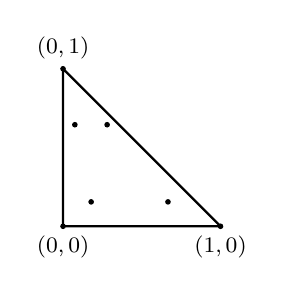
\begin{tikzpicture}[scale=2]

        \draw[thick] (0,0) -- ++(0,1) -- ++(1,-1)--cycle;
        \filldraw (0,0)         circle (0.4pt);
        \filldraw (0,0) ++(1,0) circle (0.4pt);
        \filldraw (0,0) ++(0,1) circle (0.4pt);
        \fill[black,font=\footnotesize] (0,0)         node[below] {$(0,0)$}
                                        (0,0) ++(0,1) node[above] {$(0,1)$}
                                        (0,0) ++(1,0) node[below] {$(1,0)$};
        \filldraw (0.666390, 0.155051) circle (0.4pt);
        \filldraw (0.280020, 0.644949) circle (0.4pt);
        \filldraw (0.178559, 0.155051) circle (0.4pt);
        \filldraw (0.075031, 0.644949) circle (0.4pt);
\end{tikzpicture}
\caption{Visualisation of nodes in $\hat{T}$(order 3)}\label{ch_quad_nodes_T_hat}

\end{figure}